\documentclass{semdoc}
\usepackage{subcaption}
\usepackage[export]{adjustbox}
\usepackage{graphicx}
\graphicspath{ {images/} }
% Template: $Id: t01_txt.tex,v 1.7 2000/05/23 12:13:37 bless Exp $
% -----------------------------------------------------------------------------
%epstopdf ermöglicht, dass eps-Dateien durch pdflatex in windows eingebunden werden können
%\usepackage{epstopdf}
% Report Praktikum
% -----------------------------------------------------------------------------
% Kommentare beginnen mit einem %-Zeichen
\docbegin
% --> Oberhalb der Linie bitte nichts ändern.
% ---------------------------------------------------------------------------
% \/ \/ \/ \/ \/ \/ \/ \/ \/ \/ \/ \/ \/ \/ \/ \/ \/ \/ \/ \/ \/ \/ \/ \/ \/
% Stellen, an denen etwas geaendert werden soll, sind wie hier gekennzeichnet.
% /\ /\ /\ /\ /\ /\ /\ /\ /\ /\ /\ /\ /\ /\ /\ /\ /\ /\ /\ /\ /\ /\ /\ /\ /\

%
% ---------------------------------------------------------------------------
% \/ \/ \/ \/ \/ \/ \/ \/ \/ \/ \/ \/ \/ \/ \/ \/ \/ \/ \/ \/ \/ \/ \/ \/ \/
% --> Bitte den Titel des Beitrages in die nächste Zeile eintragen:
\title{Praktikumsbericht 4}
%
% --> ... und den Namen des Autors:
\author{Jean-Marc Hendrikse - 1751591}
% /\ /\ /\ /\ /\ /\ /\ /\ /\ /\ /\ /\ /\ /\ /\ /\ /\ /\ /\ /\ /\ /\ /\ /\ /\
% -----------------------------------------------------------------------------

% Nicht ändern!
\event{Access Control Systems Lab\\}
\term{Sommersemester 2017}
\supervisor{Prof. Dr. Hannes Hartenstein, Alexander Degitz, Jan Grashöfer, Till Neudecker}

%
%
\maketitle

\section*{Einleitung} % in die Klammern die Ueberschrift
\label{Introduction} % und ein Label

In diesem Bericht stellen wir den Umgang mit \textit{Microsoft Azure} vor. Microsoft Azure (oder auch nur \textit{Azure}) ist eine Cloud-Computing-Plattform der Firma Microsoft \footnote{\url{https://www.microsoft.com}}. Es bietet Dienste wie \textit{SQL Azure} oder \textit{AppFabric} an. Hauptsächlich wird bei Azure auf \textit{Infrastructure as a Service} (IaaS), \textit{Platform as a Service} (PaaS) und \textit{Software as a Service} (SaaS) gesetzt \footnote{\url{https://de.wikipedia.org/wiki/Microsoft_Azure}}. \\
Nachdem wir ein neues Microsoft-Konto über \url{https://account.microsoft.com/account} erstellt haben und ein konstenloses Azure-Konto angelegt haben, können wir damit beginnen uns tiefer mit Azure zu befassen und uns mit dem Umgang besser vertraut machen. Dafür erstellen wir zunächst ein \textit{Windows Server 2012 R2 Datacenter} im Azure Portal und installieren \textit{Microsoft Remote Desktop}, falls dieser nicht bereits vorher auf dem System vorhanden ist. Bei der Erstellung des Windows Server wird eine \texttt{rdp}-Dtaei (in unserem Fall \texttt{DC.rdp}) generiert, die wir über Remote Desktop ausführen können. Dadurch erhalten wir Zugriff auf unseren Windows Server 2012 und können auf einem blanken System konfigurationen und Installationen durchführen. Diese blanke Version des Windows Servers dient uns als Basuis für weitere Konfigurationen. So wollen wir zum einen in Kapitel~\ref{dc} den Domain Controller näher vorstellen, der das Herzstück der Active Directory Domain Services bildet, und in Kapitel~\ref{aadc} installieren wir zur Verzeichnissynchronisation \textit{Azure Active Directory Connect}.

\section{Domain Controller}
\label{dc}

Seit der Windows Server Version 2008 ist der klassiche Active Directory (AD) in Rollen unterteilt. Die Kernkomponente bildet die Server-Rolle \textit{Active Directory Domain Services} (\textbf{AD DS}). Mithilfe des AD DS können Administartoren Informationen zu Ressourcen eines Netzwerkes ganz einfach verwalten und in verteilten Datenbanken abspeichern \footnote{\url{http://searchwindowsserver.techtarget.com/definition/Microsoft-Active-Directory-Domain-Services-AD-DS}}. Ebenso ist das Erstellen von Hierarchien für Benutzer und Computer eines Netzwerks möglich. In der Remote Desktop Konsole installieren wir auf dem Windows Server 2012 über das Tool \textit{Server Manager} nun genau diesen Dienst.\\
Im ersten Schritt legen wir drei Benutzer, zwei Gruppen und zwei Zugriffsberechtigungen (engl. \textit{permissions}) auf eine Datei an. Da wir noch keiner Domäne angehören, machen wir das nicht über das AD, sondern stattdessen lokal über das \textit{Computer Management}, das wir über \textit{Tools > Computer Management} erreichen und dort User und Gruppen verwalten. Wir legen zunächst mit einem Standardpasswort versehen drei lokale Benutzer an: \textit{Test1}, \textit{Test2} und \textit{Test3}. Außerdem legen wir die beiden Gruppen \textit{Testgroup12} und \textit{Testgroup13} an, denen wir jeweils Benutzer zuordnen. In der Gruppe \textit{Testgroup12} tragen wir die Benutzer \textit{Test1} und \textit{Test2} ein und in der Gruppe \textit{Testgroup13} werden die beiden Benutzer \textit{Test1} und \textit{Test3} hinzugefügt. Jetzt haben wir Dummy-Benutzer und -Gruppen, mit denen man Zugriffsentscheidungen sehr gut simulieren kann. In dem \textit{Dokumenten}-Ordner des angemeldeten Admin-Benutzers legen wir eine Datei namens \texttt{access\_test.txt} an. Über Rechtsklick gelangen wir über \textit{Properties > Security} auf die Operationsrechte (\textit{permissions}) für jeden einzelnen Nutzer oder jede Gruppe auf diese Datei. Initial sind die Gruppen und Nutzernamen, die auf dieser Datei operieren können, relativ unspektakulär, da lediglich der Nutzer, der die Datei erstellt hat, sowie das SYSTEM als auch alle Administratoren Berechtigungen besitzen. Um dies zu ändern, editieren wir die Benutzer und Gruppen über \textit{Edit}, wodurch sich ein zweites Fenster öffnet. In dem zweiten Fenster können wir über \textit{Add} Benutzer zur Liste der Gruppen und Benutzer hinzufügen oder aber auch herauslöschen (\textit{Remove}). Erfreulicherweise unterstützt die Eingabe eine Suchfunktion, die über das gesamte Benutzerverzeichnis sucht, sodass wir nur den Namen des Benutzers oder der Gruppe eingeben müssen und mittels \textit{Enter} die Verknüpfung hinzugefügen. Unter der Liste mit Gruppen und Benutzern befindet sich ein weiteres Feld, in dem wir die Zugriffsberechtigungen eines Benutzers oder einer bestimmten Gruppe ändern können. Zum Beispiel fügen wir der Liste die Benutzer \textit{Test1} und \textit{Test2} sowie die Gruppe \textit{Testgroup13} hinzu. \textit{Test1} bekommt Lese- und Schreibbererechtigungen, wohingegen \textit{Test2} lediglich nur eine Leseberechtigung erhält. Der \textit{Gruppe13} räumen wir eine Leseberechtigung ein. Beim durchführen eines Zugriffstests mit den jeweiligen Benutzern treffen genau diese Einstellungen zu: \textit{Test1} darf sowohl lesen als auch schreiben, \textit{Test2} darf nur lesen, aber nicht schreiben, \textit{Test3} darf, aufgrund der Gruppen-Berechtigung, lesen. Die Gruppen-Berechtigung greift nicht für Benutzer \textit{Test1}, da die Zugriffsberechtigungserteilung auf den Benutzer stärker ist als die der Gruppe.\\

\begin{figure}[h]
    \centering
    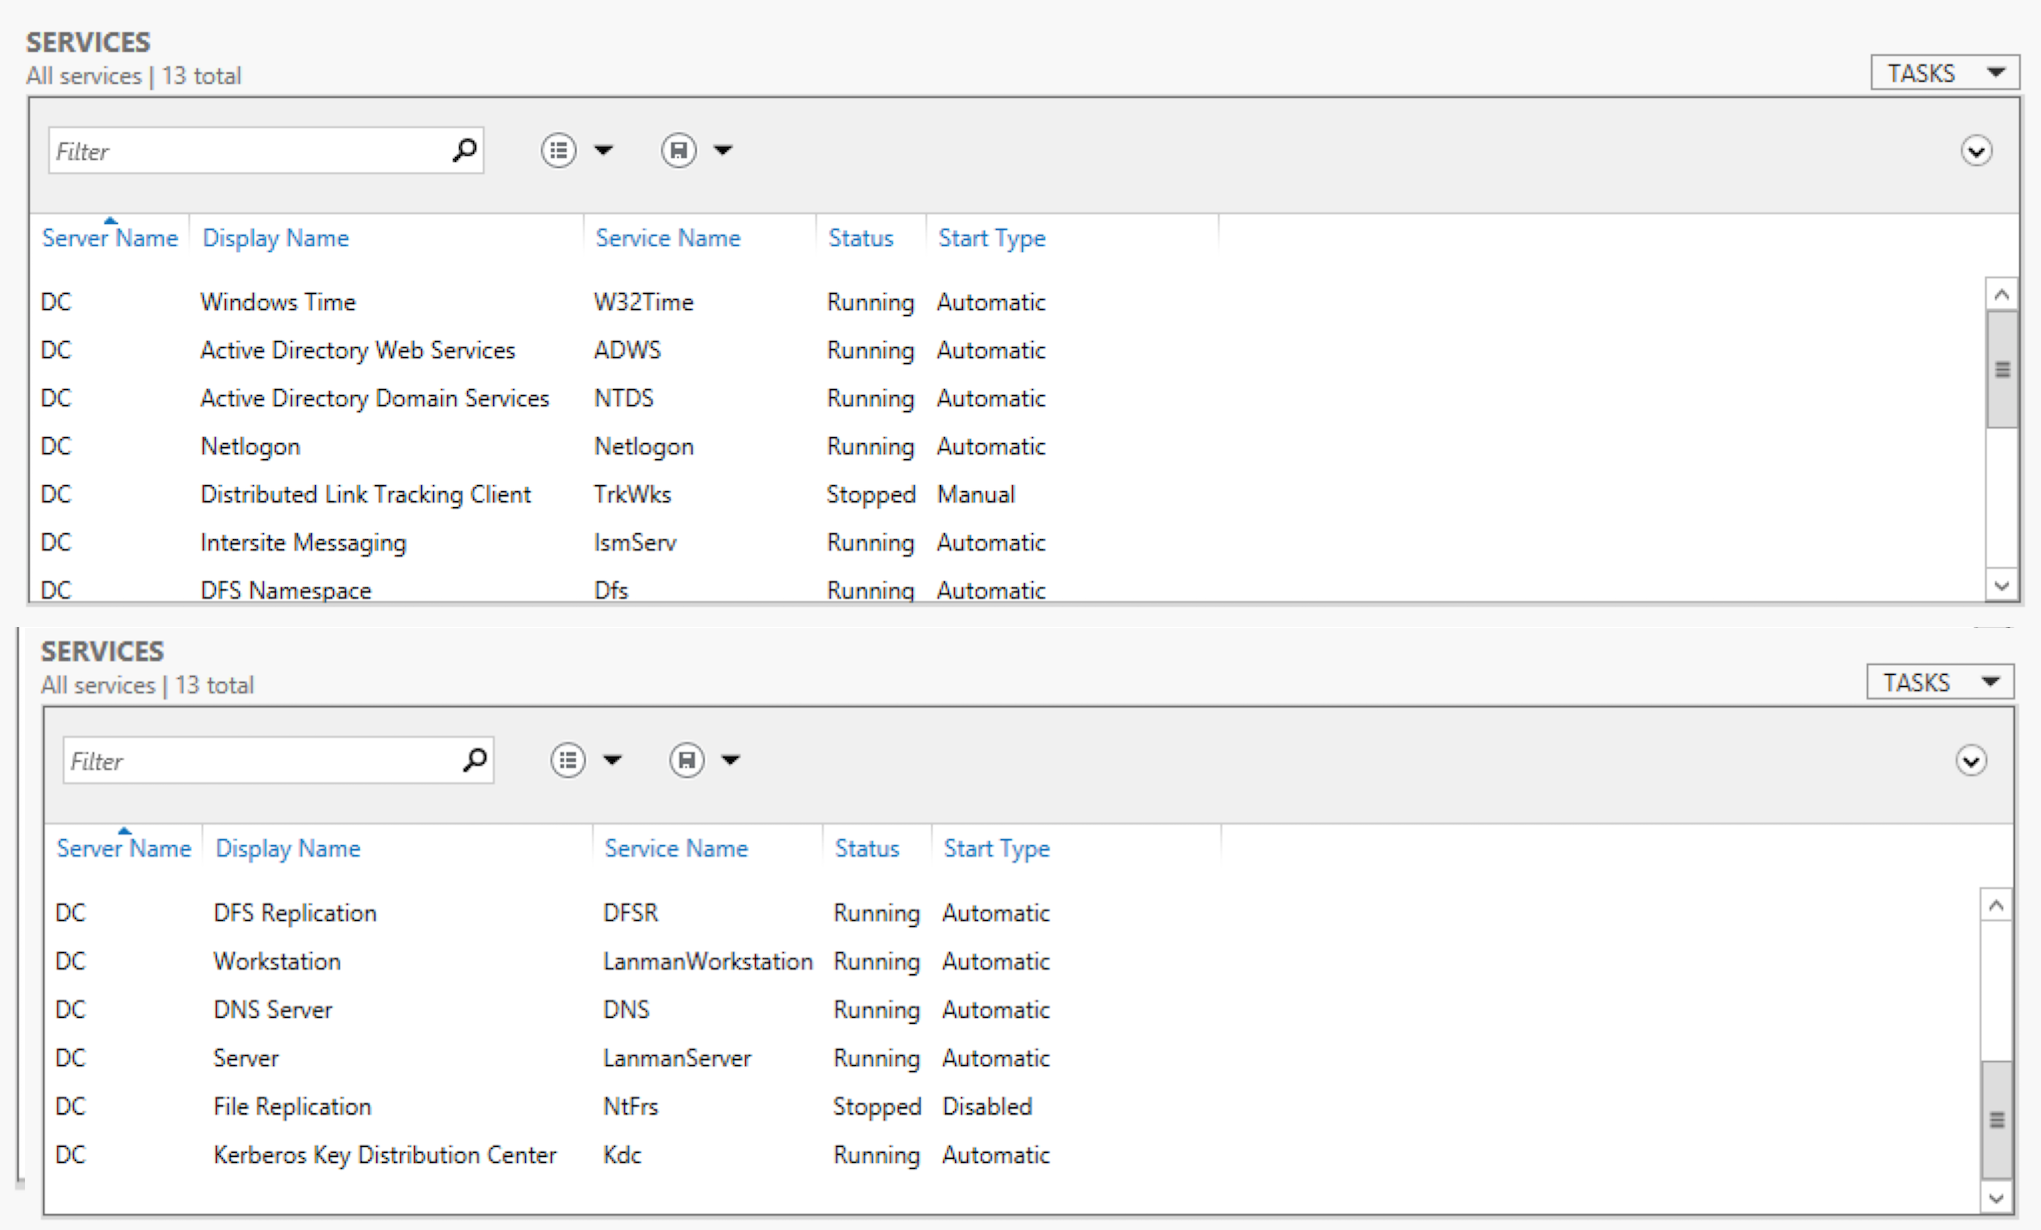
\includegraphics[width=0.8\textwidth]{Service_dependencies1}
    \caption{Services, von denen AD DS abhängt}
    \label{Bild1}
\end{figure}


Fahren wir nun weiter mit dem \textit{Domain Controller} fort: Der \textit{Domain Controller} ist eine Rolle auf dem Windows Server, der dazu dient Informationen über Benutzerkonten zu speichern, Benutzer zu authentifizieren und Sicherheitsregeln einer Windows-Domäne durchzusetzen. Computer innerhalb einer Domäne, die als Server agieren, können eine von zwei Rollen innehaben: Entweder sie haben die Rolle \textit{Member Server} oder aber \textit{Domain Controller} \footnote{\url{http://www.webopedia.com/TERM/D/domain_controller.html}}. Der \textit{Domain Controller} bildet somit das Herzstück des \textit{Active Directory Domain Service} in einem Netzwerk. Alle weiteren Services, von denen \textit{Active Directory Domain Services} abhängt, können in den Eigenschaften des AD DS gefunden werden (siehe Abbildung \ref{Bild1}). Darunter zählen Beispielsweise der DNS Server (wird zur Identifikation von Domain Controllern benötigt)\footnote{\url{https://docs.microsoft.com/de-de/azure/active-directory-domain-services/active-directory-ds-admin-guide-administer-dns}}, File Replication Service (dient zur Replikation von System-Policies) \footnote{\url{https://technet.microsoft.com/en-us/library/cc978206.aspx}}, Intersite Messaging, Key Distribution Server, Net Logon (benutzt DNS Server zur Unterstützung, um eine Registrierung von Domain Controller im DNS Domain Namespace zu ermöglichen) \footnote{\url{http://www.windowsnetworking.com/kbase/WindowsTips/WindowsServer2008/AdminTips/ActiveDirectory/FunctionsOfNetLogonServiceOnDomainControllers.html}}.

\subsection{Installation des Domain Controllers}
\label{installdc}
Bei der Konfiguration des AD Domain Services werden wird durch einen Wizard geleitet.
\begin{enumerate}
\item Deployment Configuration
\begin{enumerate}
\item In diesem Schritt Legen wir einen neuen Forest an und geben hierfür den Namen der Root-Domäne ein: in unserem Fall ist es die Root Domäne \texttt{acslab.local} (siehe Abbildung \ref{deployment_config}).
\end{enumerate}
\begin{figure}[h]
    \centering
    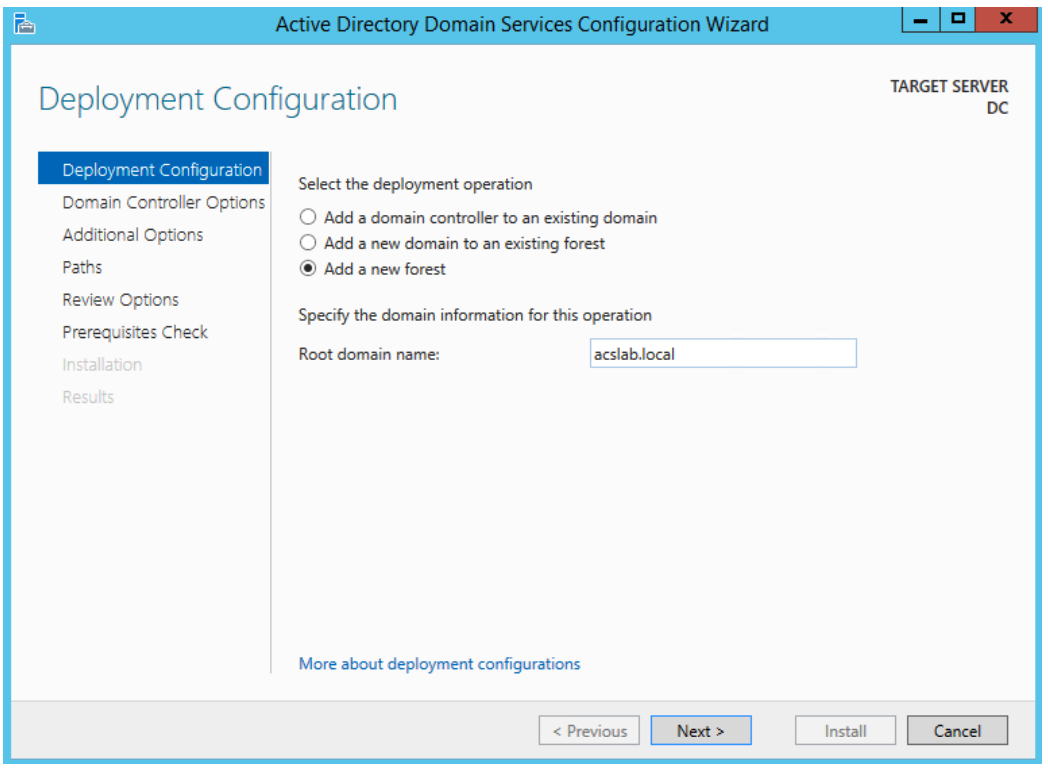
\includegraphics[width=0.8\textwidth]{deployment_config}
    \caption{Die Deployment-Konfiguration ist der erste Schritt zur Installation des Domain Controller}
    \label{deployment_config}
\end{figure}



\item Additional Options
\begin{enumerate}
\item Da wir im Forest die Domäne \texttt{acslab.local} angelegt haben, ist in diesem Schritt die NetBIOS-Domäne ebenfalls \texttt{ACSLAB}.
Die restlichen Vorkonfigurationen stimmen überein und müssen nicht weiter angepasst werden, sodass wir die Installation mit \textit{Install} abschließen können (siehe Abbildung \ref{additional_options}).
\end{enumerate}
\begin{figure}[h]
    \centering
    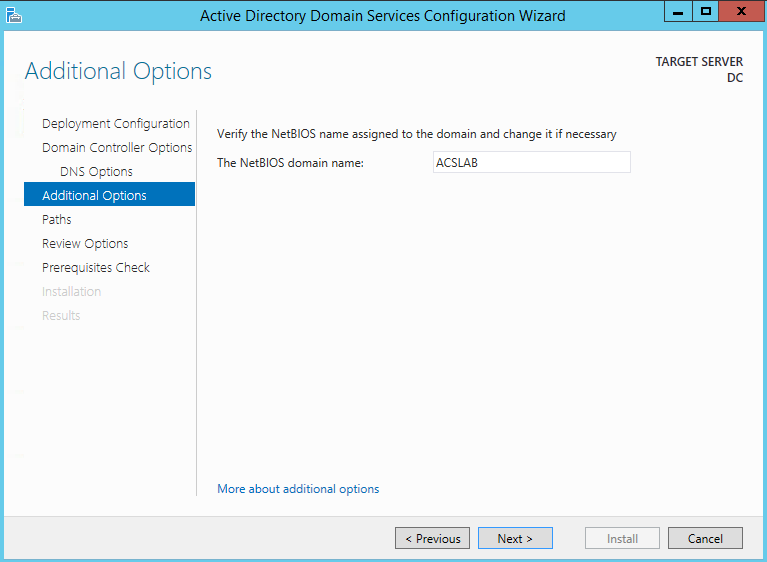
\includegraphics[width=0.8\textwidth]{additional_options}
    \caption{Additional Options für den Active Directory Domain Service}
    \label{additional_options}
\end{figure}
\end{enumerate}



\section{Verzeichnissynchronisation mit Azure Active Directory Connect}
\label{aadc}

In diesem Abschnitt wollen wir \textit{Azure AD Connect} installieren, um somit lokale Verzeichnisse in Azure Active Directory (Azure AD) zu integrieren. Das hat vor allem den Vorteil, dass wir unseren Benutzern eine Identität für alle in Azure AD integrierten Office-, Azure- und SaaS-Anwendungen bereitstellen können \footnote{\url{https://docs.microsoft.com/de-de/azure/active-directory/connect/active-directory-aadconnect}}.

\subsection{Installation von Azure AD Connect}

Zur Installation von Azure AD Connect laden wir das Tool unter \url{https://www.microsoft.com/en-us/download/details.aspx?id=47594} herunter. In den meisten Fällen besitzt man eine autorisierte lokale Domäne und kann Azure AD Connect über das Azure Portal Dashboard herunterladen und einfach installieren. In unserem Fall handelt es sich jedoch um eine Testumgebung (und nicht um eine Produktionsumgebung), sodass wir das Tool unter der zuvor genannten offiziellen URL von Microsoft herunterladen müssen. Auch hier wird man wieder über einen Wizard durch die Installation geleitet.
\begin{enumerate}
\item Dadurch, dass wir allerdings noch keinen Administrator zu unserer Domäne hinzugefügt haben, lege wir zunächst einen globalen Administrator im Azure Portal Dashboard an und vergeben ihm die Rolle \textit{Global Administrator}.
\item  Nachdem wir einen Administrator angelegt haben, können wir im Installationsschritt \textit{Connect to Azure} dessen Credentials eingeben und uns mit Azure AD verbinden.
\item Unter \textit{Domain/OU Filtering} geben wir im Verzeichnis unseren Forest-Namen \textit{acslab.local} ein und wählen die Synchronisation mit allen Domänen und OUs aus.
\item In unseren On-Premises Verzeichnissen sollen Benutzer nur einmal entlang aller Verzeichnisse repräsentiert werden und so auch identifiziert werden.
\item Das Filtering wird so gesetzt, dass alle Benutzer und Geräte entlang unseres Forest synchronisiert werden.
\item Abschließend können wir auswählen, dass während der Installation/Konfiguration alle Services auf dem Server synchronisiert werden.
\end{enumerate}

Die größten Herausforderungen die sich hierbei ergaben, war zu erkennen welche Domäne als lokale Domäne eingetragen werden soll und welcher Nutzer sich mit Azure AD verbinden muss. Dabei kann man aber relativ schnell erkennen, dass der vorherangelegte Forest als Root Domäne eingetragen werden kann und im Azure Portal ein neuer Benutzer mit globalen Administratorrechten angelegt werden muss.
Ist die Installation abgeschlossen und wurden alle Services automatisch während des Installationsprozesses synchronisiert, kann über das Azure Portal eingesehen werden, dass alle Benutzer-Konten aus dem lokalen Verzeichnis angelegt wurden. Vorher tauchten diese nämlich nicht im Azure Portal auf. \\
Möchte man jetzt weitere Benutzer in der Domäne anlegen geht man nicht wie vorher über das lokale Server Managament sondern dieses mal über die Active Directory. Nennen wir einen neuen Benutzer Test4, geben ihm ein Standard passwort und fügen ihn der Domäne \texttt{acslab} hinzu (vergleiche dazu Abbildung \ref{add_user_in_add}. Im Azure Portal ändert sich allerdings zunächst nichts. Das ist auch klar, da wir noch keine Synchronisation angestoßen haben. Nachdem wir den Befehl \texttt{Start-ADSyncSyncCycle -PolicyType Delta} in der Powershell eingeben (Abbildung \ref{powershell}), taucht der neue Benutzer im Azure AD auf.

\begin{figure}[h]
    \centering
    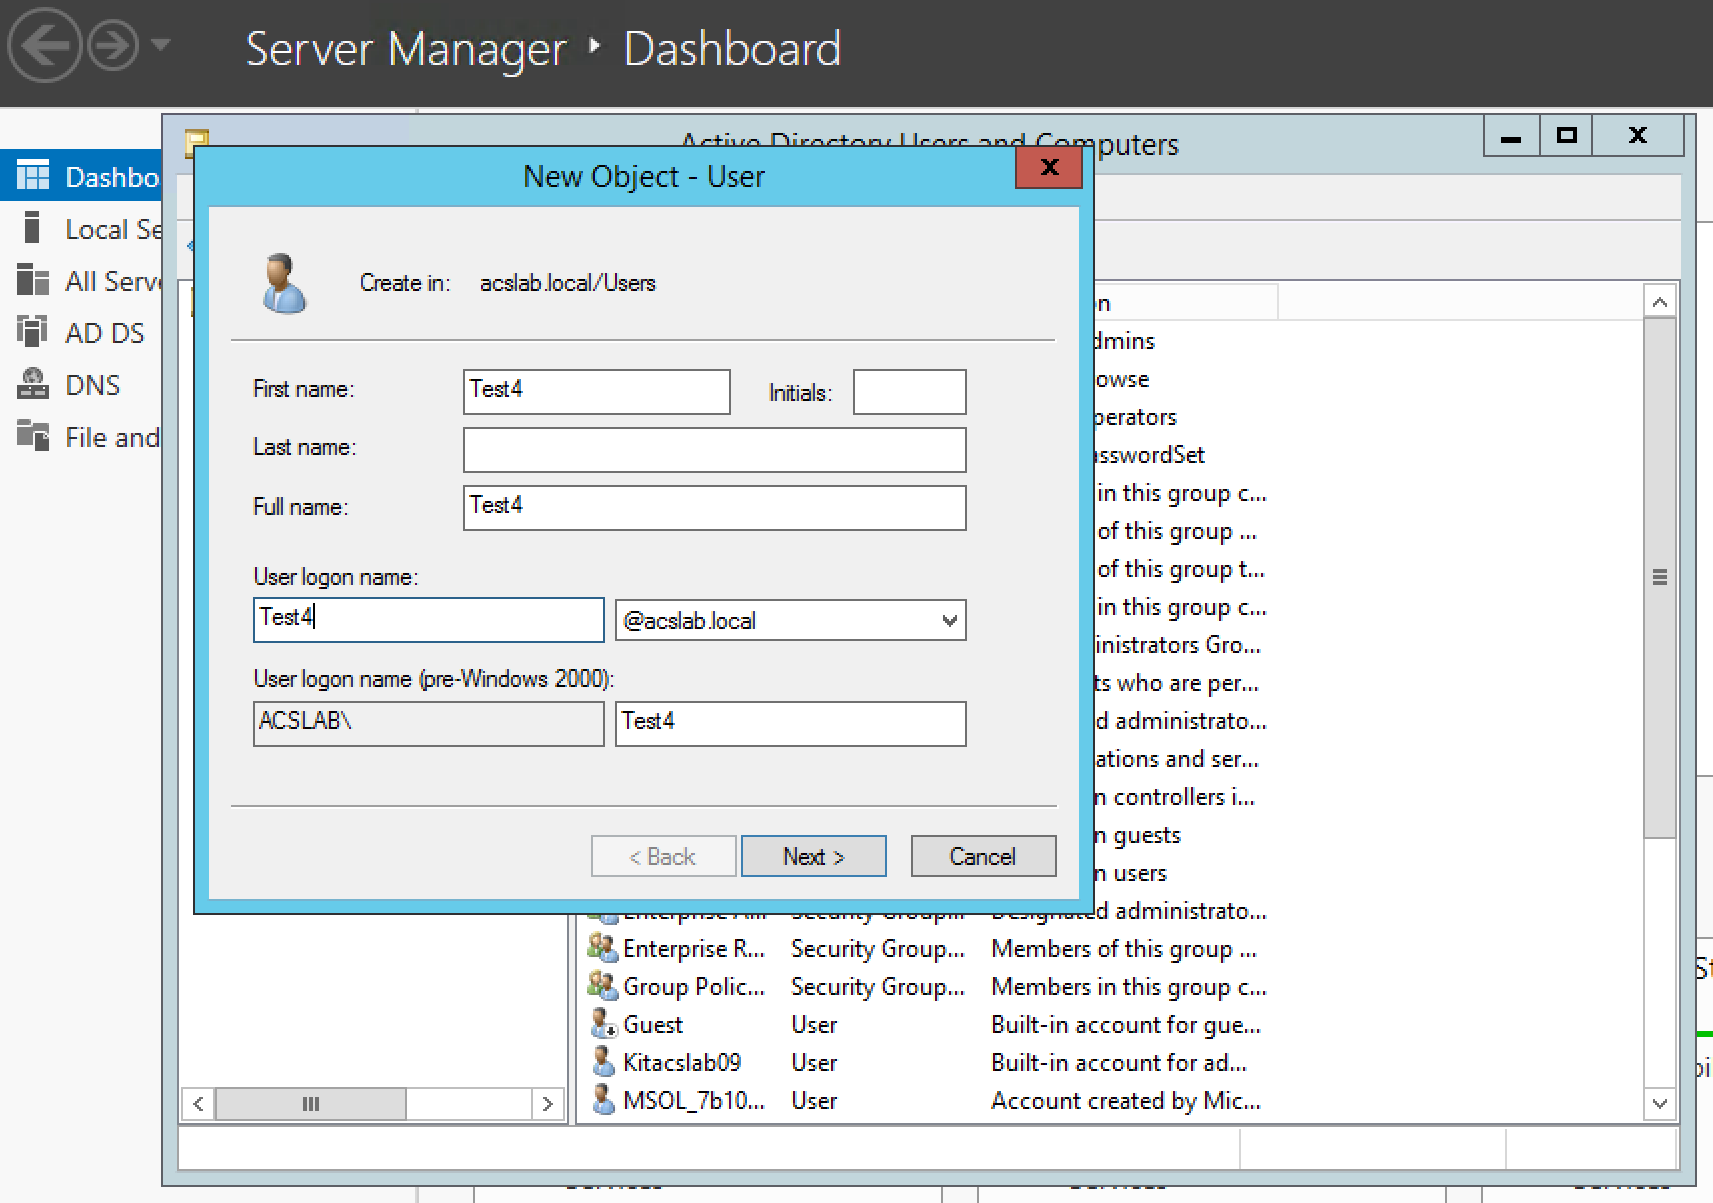
\includegraphics[width=0.8\textwidth]{add_user_in_add}
    \caption{Hinzufügen eines Benutzers Test4 im AD.}
    \label{add_user_in_add}
\end{figure}

\begin{figure}[h]
    \centering
    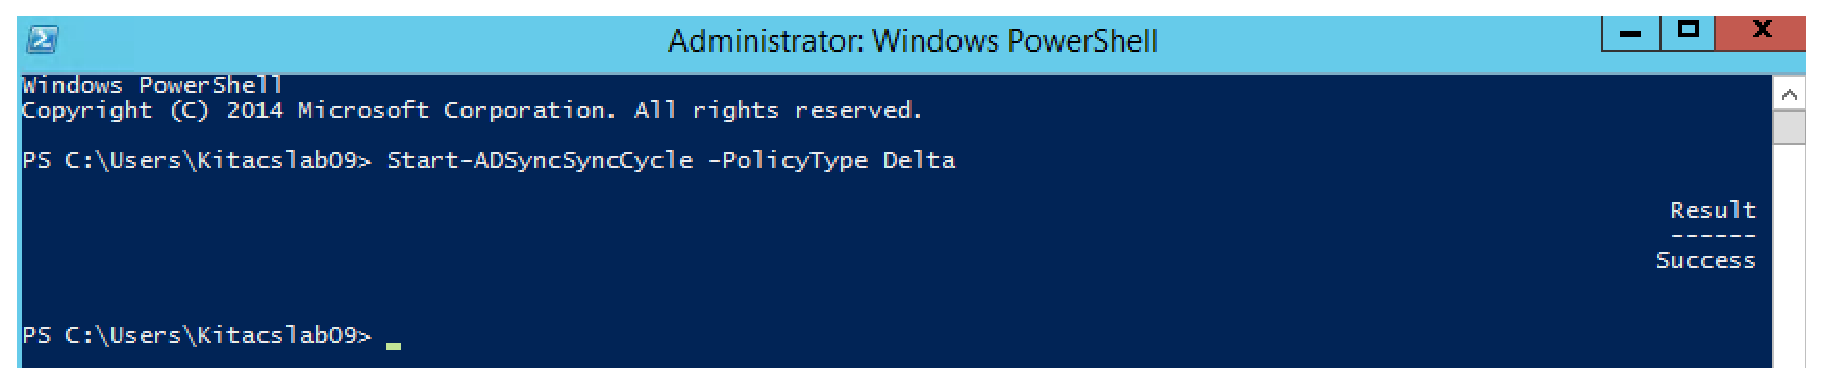
\includegraphics[width=0.8\textwidth]{powershell}
    \caption{Komando zum Starten der Synchronisation über die Powershell.}
    \label{powershell}
\end{figure}

\section{Fazit und Diskussion}
\label{conclusion}

Über wenige Konfigurationsschritte und Installationen kann mittels Microsoft Azure eine gute und für den allgemeinen Anwendungsfall angemesse Lösung zur Synchronisation von Verzeichnissen ermöglicht werden. \\
Einer der größten Vorteile, der sich durch die Integration lokaler Verzeichnisse in Azure AD ergibt, ist, dass Benutzer für Zugriffe auf Cloud-Dienste wie Office 365 als auch auf lokale Ressourcen nur eine einzige Identität benötigen. Somit müssen sie sich auch nur ein Passwort merken, das wiederum dem Vergessen von Passwörtern entgegenwirkt.
Ebenfalls erleichtert die Synchronisation den administrativen Aufwand, da eine konsistente Passwort-Policy leichter entworfen werden kann und keine User-Workstations angepasst werden müssen.  \\
Nachteile, die sich allerdings mit der Passowort-Synchronisation und der Identitätsverwaltung ergeben sind zum einen, dass dabei auch die Wahrscheinlichkeit steigt, dass Passörter kompromittiert werden. Damit kann derjenigen mit kompromittierten Passwort auf Systeme zugreifen, die mit dem Passwort synchronisiert sind. Es gibt immer noch Systeme, die eine bi-direktionale Passwortsynchronisation nicht unterstützen. Weiterhin greifen auch Passwort-Policies längst nicht auf allen System wie es die Theorie vorsieht. Somit wird eine zentrale Verwaltung der Passwort-Policies ineffizient, da er mit einem größerer Implementierungsaufwand verbunden ist. Hinzukommt, dass die Synchronisation von Identitäten leider nicht eine sichere und prüfbare Lösung für administrative, super-user oder privilegierte Identitäten bereitstellt.\footnote{\url{https://www.rsconnect.net/en/articles/pros-cons-active-directory-password-synchronisation/}}


\begin{thebibliography}{9}
\bibitem{ms}
  \urltext{https://www.microsoft.com}
\bibitem{wiki}
  \urltext{https://de.wikipedia.org/wiki/Microsoft\_Azure}
\bibitem{sws}
  \urltext{http://searchwindowsserver.techtarget.com/definition/Microsoft-Active-Directory-Domain-Services-AD-DS}
  \bibitem{wp}
  \urltext{  http://www.webopedia.com/TERM/D/domain\_controller.html}
  \bibitem{msdoc}
  \urltext{https://docs.microsoft.com/de-de/azure/active-directory-domain-services/active-directory-ds-admin-guide-administer-dns}
  \bibitem{techms}
  \urltext{https://technet.microsoft.com/en-us/library/cc978206.aspx}
    \bibitem{wn}
  \urltext{http://www.windowsnetworking.com/kbase/WindowsTips/WindowsServer2008/AdminTips/ActiveDirectory/FunctionsOfNetLogonServiceOnDomainControllers.html}
    \bibitem{msdocsa}
  \urltext{https://docs.microsoft.com/de-de/azure/active-directory/connect/active-directory-aadconnect}
\bibitem{pros}
  \urltext{https://www.rsconnect.net/en/articles/pros-cons-active-directory-password-synchronisation/}

\end{thebibliography}
%
\docend
%%% end of document
